

An additional task of monitoring the data quality of the
electromagnetic calorimeter was conducted during the PhD, this task is
described here. A good quality of data for the \Gls{ECal} is required
for the both analyses described in this thesis, as will be described
later. Both the analyses (Neutral Current single photon search and
\Gls{ND} electron (anti-) neutrino selection) use the \Gls{ECal} for
vetoing events and the \Gls{ND} electron (anti-) neutrino selections
uses the \Gls{ECal} for particle identification.

To ensure that the quality of the data is good for all the components
of the experiment, checks are realised by the beam, \Gls{ND} and
\Gls{SK} groups.  For the \Gls{ND}, each sub-detector is checked
individually by a data quality expert who produces monitoring plots
every week during the period of data taking and when the detector is
powered on. In the case of the \Gls{ECal}, the main quantities that
are checked are the timing, the gains, the pedestals and the event
rates, which are checked at the end of each run.

As shown in Section~\ref{subsubsec:ecal}, the \Gls{ECal} encompasses
different detectors in the \Gls{ND}. The readouts for these are all
separated into 12 Read-out Merger Modules (\Gls{RMM}) which are
collecting data from a total of 366 Trip-T Front-end Boards
(\Gls{TFB}). These \Glspl{TFB} are directly connected to each channels
(Multi-Pixel Photon counter, \Gls{MPPC}). Typically, the checks are
divided for each \Gls{RMM} and each of them is checked individually.

Once the normal operation has been established for all the
\Glspl{RMM}, a flag is uploaded to a SQL database which is later used
for processing the data. Each \Gls{RMM} is treated independently.  The
flag is a 12 bit field translated to decimal number which is assigned
between two timestamps. During the normal running of the \Gls{ECal},
the flag will be 0 (or 000 000 000 000 in the binary basis), whilst if
a \Gls{RMM} is not working normally the flag will be equal to
$2^{\text{RMM}}$. If several \Glspl{RMM} are not working properly then
the sum of these numbers will be the flag\footnote{For example, if
  \Gls{RMM}2, 3 and 11 were not working normally the bit field will
  be: 100 000 001 100, which translates to $2^{11}+2^{3}+2^{2}=2060$
  in the decimal basis.}

This task has been carried out for the 12 \Glspl{RMM} of the
\Gls{ECal} during two years. For the purpose of clarity, only the run
7 \Gls{RMM}0 data (which is the 2016 data of half of the
\Gls{DsECal}), is shown in this section, unless stated otherwise.

In the first section, the beam timing monitoring is explained; then
the monitoring of gain and pedestal are described. Finally, the
stability of event rates is demonstrated in the last section. This
section shows that the \Gls{RMM}0 of the \Gls{ECal} (and more
generally the whole \Gls{ECal}) has produced good and usable data for
run~7 data-taking period.


\section{Beam timing}
\label{sec:beamtiming}

The reconstruction good timing of the hits in the detector are
required to be able to match the track between the \Gls{ND}
sub-detectors. Knowledge of the beam timing in the \Gls{ECal} relies
on the offsets introduced by the electronics, which can be simulated.

In Figure~\ref{fig:beamtiming}, one can see some examples of timing
distributions. In this figure, one clearly sees the bunch structure of
the beam.

The blue bands are the \Gls{ECal} reset windows between each bunch. It
can happen that the high voltage fluctuates and introduces some
variations in the beam timing profile. For run 7, this has been very
rare and it is believed that all the fluctuations in these histograms
are due to changes in the configuration of the beam itself rather than
in the \Gls{ECal}. For other runs, it was noted that fluctuations
could happen if the power supply of a \Gls{RMM} changes, or if a
mistake is introduced in the cabling of the \Gls{RMM} while
maintaining the detector.

\begin{figure}[ht]
  \begin{adjustbox}{center}
    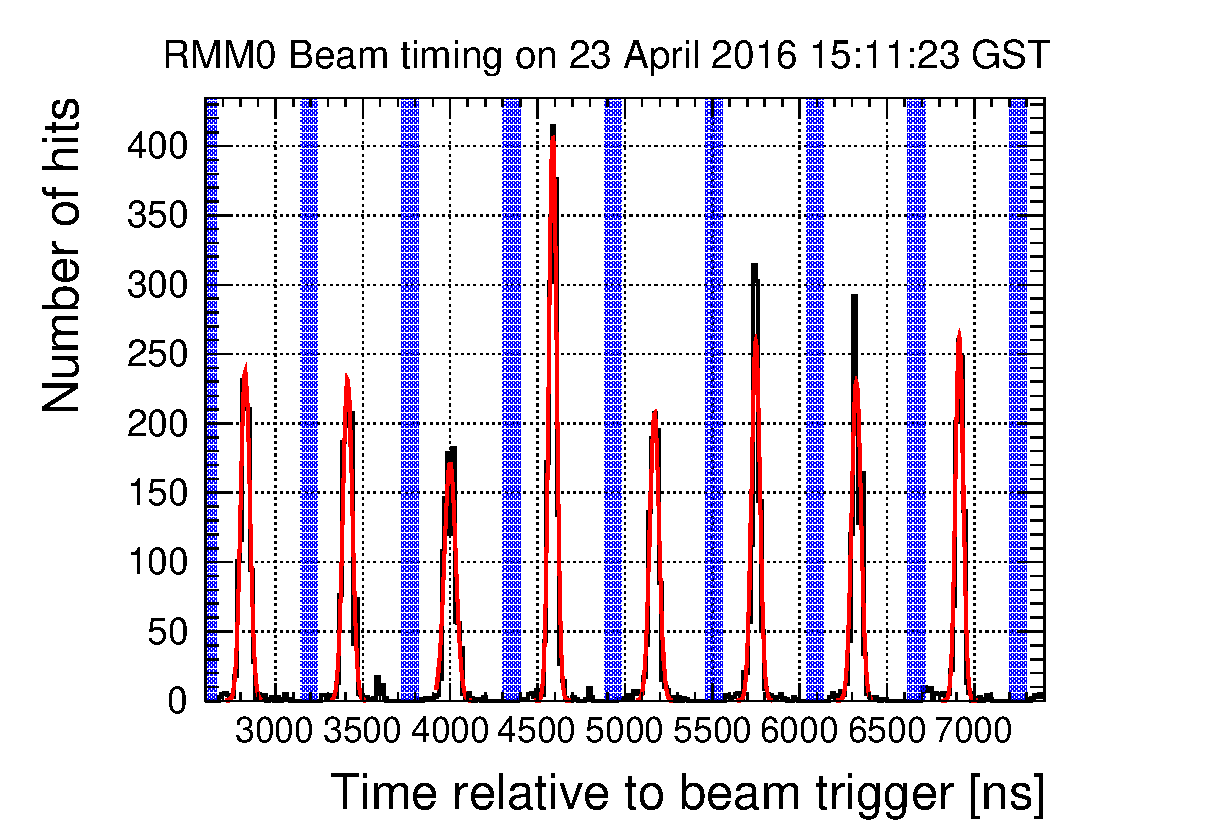
\includegraphics[width=0.48\textwidth]{images/DataQuality/BeamTimingDetail.eps}
    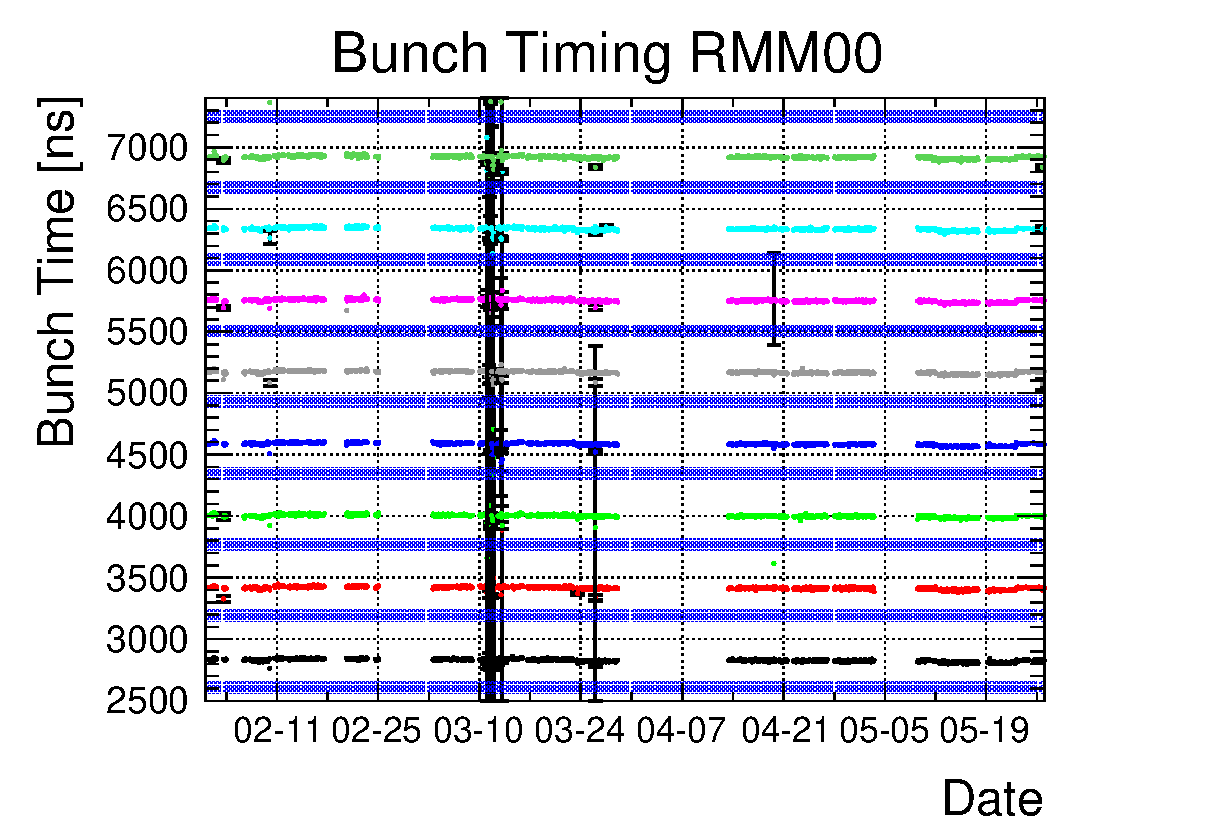
\includegraphics[width=0.48\textwidth]{images/DataQuality/BeamTimingRun7.eps} 
  \end{adjustbox}
  \caption[Run 7 beam timing data of the ECal]{\textbf{\textit{Left:}}
    Beam timing data (black) for \Gls{RMM}0 fitted by 8 Gaussian
    curves (red). \textbf{\textit{Right:}} Mean of the Gaussian fits
    over extended period for the run 7. Note that all the points with
    a large error are points for which the Gaussian fit did not
    converge properly as there were too few points to fit. The
    \Gls{ECal} reset window are in blue on both figures.}
  \label{fig:beamtiming}
\end{figure}

The check consists of producing figures such as the one on the right
of Figure~\ref{fig:beamtiming} every week, and checking that all the
points are aligned. Any deviation from constant beam timing has to be
explained and flagged accordingly.

\section{Gain and Pedestal of the MPPC}
\label{sec:gainped}

The \Gls{ECal} gains for each channel are also checked every
week. Fast and large gain variations are not desirable as they make
the calibration more complex, and can be indicative of a problem with
the \Gls{ECal} or its power supply. The \Gls{ADC}\footnote{ADC: Analog
  to Digital Converter} counts of each channel can be used to
calculate the pedestal and gain values. To do that, the \Gls{ADC}
counts are stored in a histogram over a period which corresponds to
about 20 minutes (usually 500 events). An example of the histogram is
shown in Figure~\ref{fig:DPT} for a longer period.  In this histogram,
the first peak corresponds to having no hit in the \Gls{MPPC} and is
called the pedestal. The pedestal is the \Gls{ADC} value when nothing
happens in the detector. One could manually set the pedestal value to
be read $0$ in the \Gls{ADC}, however this is not preferable because
the \Gls{ADC} is not linear in this region. The second peak
corresponds to the \Gls{ADC} output when one photo-electron fires one
pixel. The difference between the first two peaks provides a direct
measurement of the single photo-electon response, i.e. the number of
\Gls{ADC} counts for each detected photo-electron. This single
photo-electron response can be use to calculate the gain.

\begin{figure}[ht]
  \begin{adjustbox}{center}
    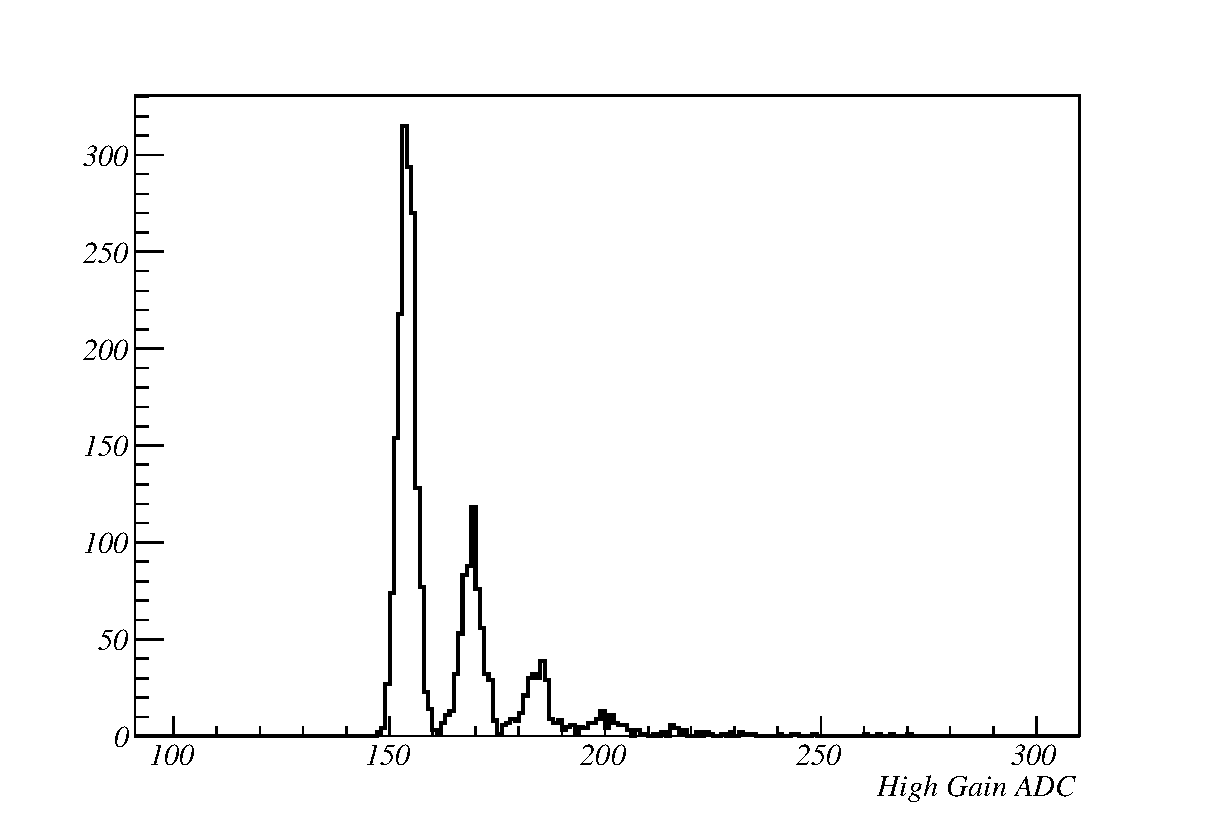
\includegraphics[width=0.8\textwidth]{images/DataQuality/highgainraw.eps}
  \end{adjustbox}
  \caption[A DPT high gain channel histogram, ECal ADC readings
  showing the first, second, third and fourth photo-electon peaks]{Few
    \Gls{ECal} \Gls{ADC} readings for the high gain channel, this
    figure is called a \Gls{DPT} (Data Processing Task) histogram. The
    histograms are realised by the processing nodes (\Gls{TFB}) by
    using the data from all the Trip-T detectors connected to the
    \Gls{TFB} during a period of around 20~min (500 events). On this
    figure, the first, second, third and fourth photo-electron peaks
    are visible from left to right. Such histograms are used during
    the calibration of the detectors. Taken from~\cite{T2KCalib}.}
  \label{fig:DPT}
\end{figure}


Every week, the value of the pedestal and gain are checked. Note that
on top of the built-in \Gls{MPPC} gain (of about $10^6$ as shown in
Subsection~\ref{subsec:mppc}), there are two electronic gain channels:
\begin{itemize}[noitemsep,topsep=0pt]
\item a high gain channel, where $1$~\Gls{PEU}\footnote{PEU: Pixel
    Equivalent Unit, is the raw value in pC of the charge detected by
    the \Gls{MPPC}.} is encoded in $\sim 10$~\Gls{ADC} counts. This
  value can be seen in the difference between the two first peaks of
  Figure~\ref{fig:DPT},
\item and a low gain channel, where a $1$~\Gls{PEU} is encoded in
  $\sim 1$~\Gls{ADC} counts.
\end{itemize}
This provides two sets of measurements relevant for many detected
photo-electrons, for the low gain channel; and few photo-electrons for
the high gain channel. For the low gain, the pedestal and the first
photo-electron peak are superimposed, and hence the equivalent of
Figure~\ref{fig:DPT} for the low gain channel would only have one
peak. This means the only gain that can be easily monitored is the
high gain. It is also the most sensitive one.

To produce the weekly plots used for the monitoring, on
Figures~\ref{fig:gain} and \ref{fig:ped}, a reference value of the
gain is taken every time calibration is done (typically once every
week). Then, the difference between the gain and the reference is
``histgrammed'' over the week for all the channels. The same procedure
is applied for the high and low pedestal. The differences should be
under 0.5 in absolute value (red line).

As for the beam timing, any deviation from the allowed regions should
be understood and flagged accordingly. Since the gain are dependant on
the temperature (see Section~\ref{subsec:mppc}), it is very common
that abrupt changes of temperature cause the gain to change to
unacceptable values. This generally happens after a long shutdown,
when the \Glspl{RMM} boards are cold, when the magnet is being closed
or when the magnetic field is turned off of on. Additionally, extreme
weather variations can cause unwanted gain variations. ``Turn-on''
effects are visible on Figures~\ref{fig:gain} and \ref{fig:ped}, where
the gain and pedestal value change abruptly in the beginning of the
run or after the winter shutdown.

\begin{figure}[ht]
  \begin{adjustbox}{center}
    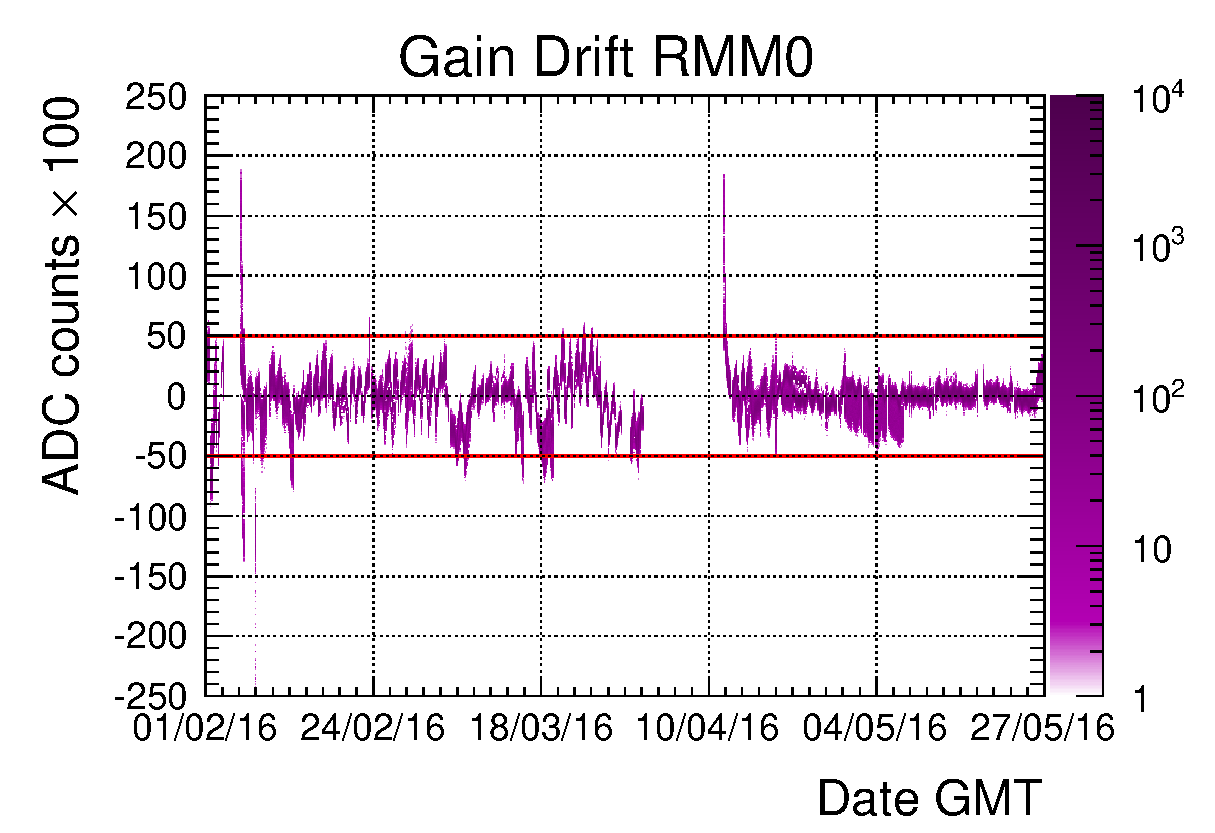
\includegraphics[width=0.58\textwidth]{images/DataQuality/gaindrift.eps}
  \end{adjustbox}
  \caption[Run 7 ECal RMM0 gain drifts]{\Gls{ECal} \Gls{RMM}0 gain
    drifts over run 7.}
  \label{fig:gain}
\end{figure}


\begin{figure}[ht]
  \begin{adjustbox}{center}
    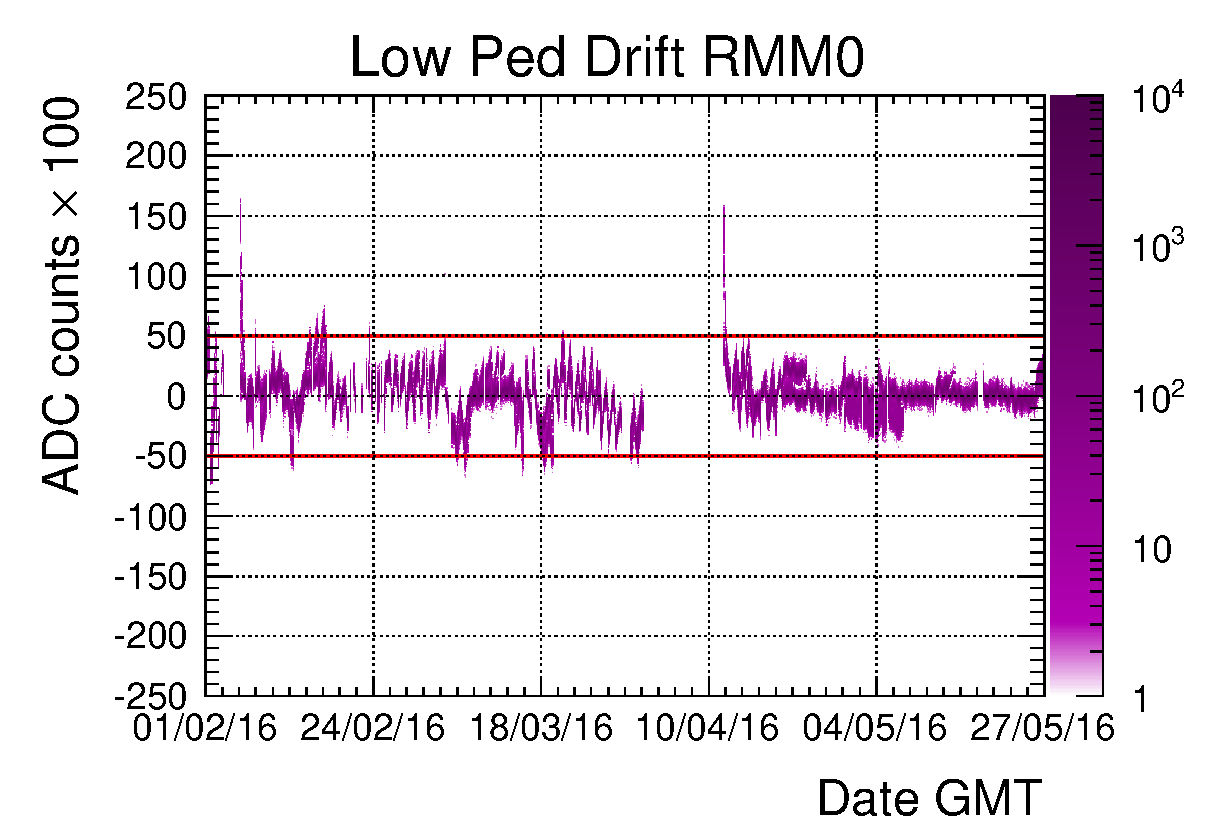
\includegraphics[width=0.48\textwidth]{images/DataQuality/lowped.eps} 
    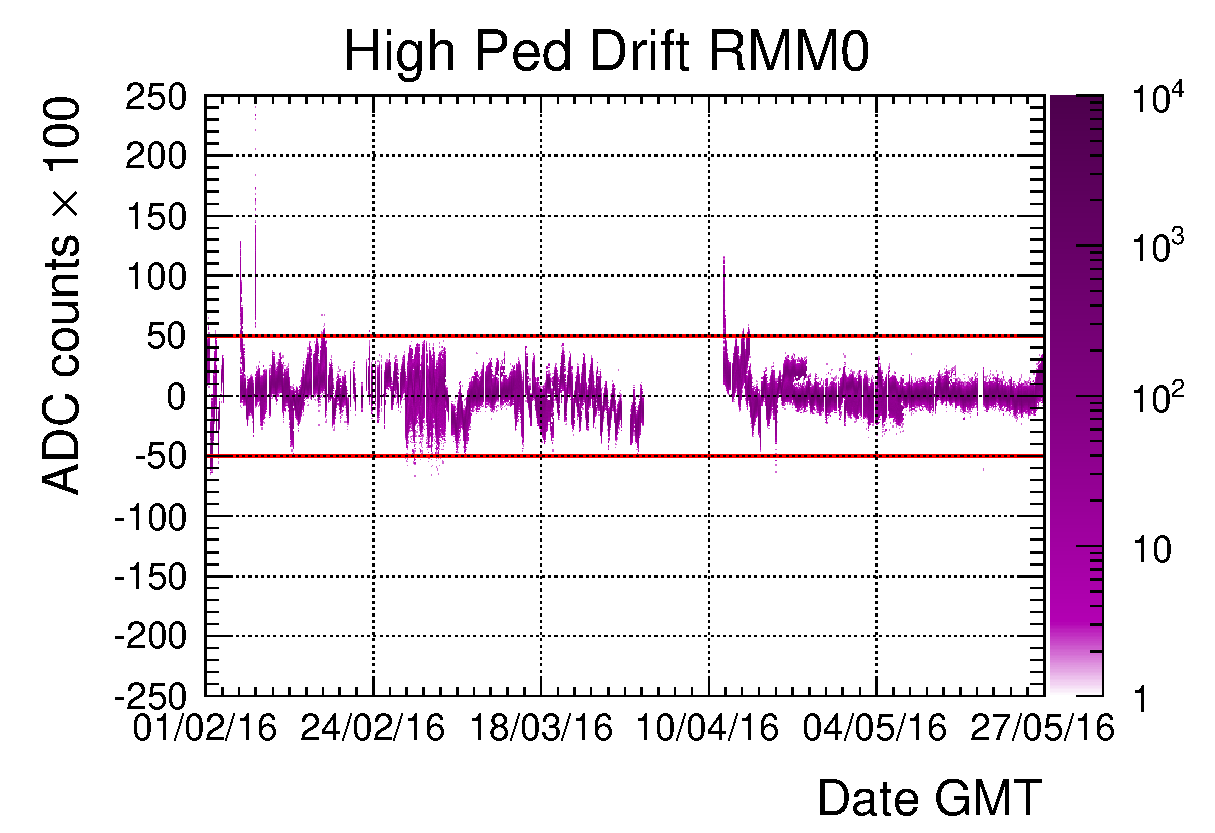
\includegraphics[width=0.48\textwidth]{images/DataQuality/highped.eps}
  \end{adjustbox}
  \caption[Run 7 ECal pedestal drifts]{\Gls{ECal} \Gls{RMM}0 pedestal
    drifts over run 7. \textbf{\textit{Left:}} Low
    pedestal. \textbf{\textit{Right:}} High pedestal.}
  \label{fig:ped}
\end{figure}

\section{Event rates}
\label{sec:eventrate}
Another final check that is realised consists in checking the event
rate of the \Gls{ECal}.  This is done once at the end of the run. To
do this, a simple cluster algorithm is run on the data. One can then
normalise the number of reconstructed clusters by the number of
\Gls{POT} (Protons on Target). If the \Gls{ECal} runs normally, this
number should be constant over time. Some changes can happen if the
horn current is modified (if the horn current increases, for example,
more neutrinos are going to be focused and reach the \Gls{ECal} thus
increasing the event rate). Similarly, if the horn polarity is
reversed, the fraction of neutrinos and anti-neutrinos reaching the
\Gls{ECal} will be different and will lead to different event
rates.

The result for run 7 is shown in Figure~\ref{fig:eventrate} (in this
figure, all the \Glspl{RMM} cluster\footnote{A cluster is defined here
  as at least three hits (i.e. at least one detected photo-electron
  for three different bars), in adjancent bars, in a time window of
  $30\text{~ns}$. The cluster is expanded from the highest detected
  charge to neighboring bars. Note that for physics purpose, the
  number of required hits is seven, which is an additional security to
  noise clusters.} rates are summed). One can see that the event rate
for anti-neutrino mode is smaller than in neutrino mode. This happens
because the both the anti-neutrino flux and cross section are much
smaller than the in the neutrino case. As can be seen, some problems
happened around mid-April, when the part of the \Gls{BrECal} was
turned off due to a cooling issue.

\begin{figure}[ht]
  \begin{adjustbox}{center}
    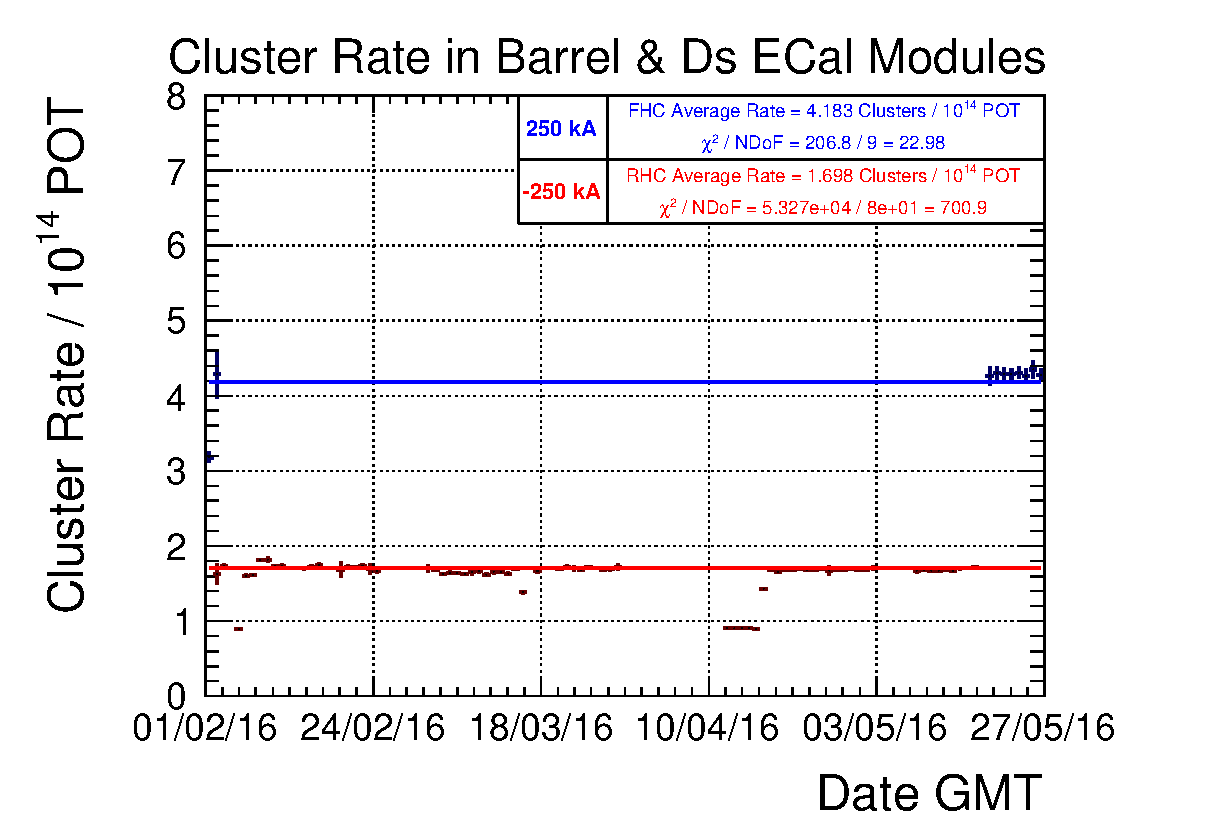
\includegraphics[width=0.7\textwidth]{images/DataQuality/ClusterRates.eps} 
  \end{adjustbox}
  \caption[Run 7 ECal cluster rate]{Cluster rate for all the
    \Gls{ECal} during run 7, during which the horn polarity was
    positive (\Gls{FHC}, in blue) and negative (\Gls{RHC}, in red).}
  \label{fig:eventrate}
\end{figure}


\section{Summary}
\label{sec:dqsummary}
From the three sections developed in this chapter, it is clear that
the \Gls{ECal} of the \Gls{ND} delivers good and usable
data. Monitoring the data quality is a fundamental step during the
data-taking periods which ensures fast feedback and diagnostic of the
problem to the expert in charge of the maintenance of the
detector. This is critical as the \Gls{TK} collaboration has to make
sure that all the allocated beam time of the experiment can be used
for physics analysis and thus address any hardware issue as fast as
possible. The \Gls{ECal} data has found many use for \Gls{ND} analyses
(high angles~\cite{TN310,TN348}, \Gls{ECal} as target
analyses~\cite{DomBrailsford2016}) which includes the two analyses
described in this thesis (\Gls{NCg} and electron (anti-) neutrino
selections).




